\documentclass{beamer}
\usepackage{booktabs}
\usepackage{pdfpages}
\usepackage{mathtools}
\usepackage{enumerate}

\PassOptionsToPackage{usenames,dvipsnames,svgnames}{xcolor}  
\usepackage{tikz}
\usetikzlibrary{arrows,positioning,automata}


\usepackage{wasysym}
\usepackage{proof}
\usepackage{cancel}
\usepackage{chronology}
\usepackage{graphicx}
\usepackage{ulem}
\usepackage{amsmath}
\usepackage{amssymb}
\usepackage{color}
\usepackage{xcolor}
\usepackage{soul}
%\usepackage{pstricks}
\setbeamertemplate{navigation symbols}{}

\newcommand{\myul}[2][blue]{\sethlcolor{#1}\hl{#2}\setulcolor{black}}

\newcommand<>{\cunderline}[3]{\only<#1>{#3}\only<#2>{\underline{#3}}}
\newcommand<>{\cem}[3]{\only<#1>{#3}\only<#2>{\ul{#3}}}
\newcommand<>{\cgray}[3]{\only<#1>{#3}\only<#2>{\textcolor{gray}{#3}}}
\newcommand<>{\colorize}[4]{\only<#1>{#4}\only<#2>{\textcolor{#3}{#4}}}

%\setbeamertemplate{navigation symbols}{}
\addtobeamertemplate{navigation symbols}{}{%
    \usebeamerfont{footline}%
    \usebeamercolor[fg]{footline}%
    \hspace{1em}%
    \insertframenumber/\inserttotalframenumber
}

\renewcommand{\em}{\itshape}

\mode<presentation>
% {
%   \usecolortheme{crane}
% %  \usetheme{Frankfurt}
% }
\mode<presentation>
{
  \usecolortheme{dove}
}

% \mode<presentation>
% {
% \useinnertheme[shadow=true]{rounded}
% \useoutertheme{infolines}
% \usecolortheme{dove}
% \setbeamerfont{block title}{size={}}
% }

\title[Bio-Ontologies]{Introduction to ontologies}
\subtitle{Semantic similarity}

\author{Michel Dumontier \& Robert Hoehndorf}


\date{ISMB 2017}

\begin{document}

\begin{frame}
  \titlepage
\end{frame}

\begin{frame}
\frametitle{Overview}
\begin{enumerate}
\item Ontologies and graphs
\item Structural similarity
\item Information theoretic approaches
\item Set-based
\item Applications
\end{enumerate}
\end{frame}

\begin{frame}
  \frametitle{Some examples}
  \begin{itemize}
  \item Are cyclin dependent kinases {\em functionally} more similar
    to lipid kinases or to riboflavin kinases? How about {\em
      phenotypically}?
    \pause
  \item Which protein in the {\em mouse} is functionally most similar
    to the zebrafish {\em gustducin} protein?
    \pause
  \item Which mouse knockout resembles {\em Bardet-Biedl Syndrome 8}?
    \pause
  \item Are there mouse knockouts that resemble the side effects of
    diclofenac?
    \pause
  \item Which genetic disease produces similar symptoms to ebola?
    \pause
  \item Does functional similarity correlate with phenotypic similarity?
  \end{itemize}
\end{frame}

\begin{frame}
  \frametitle{Ontologies and graphs}
  \begin{itemize}
  \item semantic similarity measures can be graph-based,
    feature-based, or model-based
  \item we may need to generate graphs from ontologies
    \begin{itemize}
    \item {\em is-a} relations are easy
    \item how about {\em part-of}, {\em regulates}, {\em precedes}, etc.?
    \end{itemize}
  \item relational patterns are defined in OBO Relation Ontology
    \begin{itemize}
    \item in first order logic
    \item needs to translate them into OWL
    \end{itemize}
  \end{itemize}
\end{frame}

\begin{frame}
  \frametitle{Relations as patterns}
  \begin{itemize}
  \item {\tt X SubClassOf: Y}: $X \xrightarrow{\text{is-a}} Y$
  \item {\tt X SubClassOf: part-of some Y}: $X \xrightarrow{\text{part-of}} Y$
  \item {\tt X SubClassOf: regulates some Y}: $X \xrightarrow{\text{regulates}} Y$
  \item {\tt X DisjointWith: Y}: $X \xleftrightarrow{\text{disjoint}} Y$
  \item {\tt X EquivalentTo: Y}: $X \xleftrightarrow{\equiv} Y$, $\{X,Y\}$
  \end{itemize}
\end{frame}

\begin{frame}
  \frametitle{Relations as patterns}
  \begin{itemize}
  \item OBO Relation Ontology (RO):
    \begin{itemize}
    \item \url{https://github.com/oborel/obo-relations}
    \end{itemize}
  \item Basic Formal Ontology (BFO):
    \begin{itemize}
    \item provides top-level classes
      \begin{itemize}
      \item Continuant, Process, Function, Material object, etc.
      \end{itemize}
    \item used for some OBO Foundry ontologies
    \end{itemize}
  \item RO and BFO provide a top-level system of classes and relations
    shared across many biomedical ontologies
    \begin{itemize}
    \item even GO, although somewhat hidden!
    \end{itemize}
  \end{itemize}
\end{frame}

\begin{frame}
  \frametitle{Relations as patterns}
  \centerline{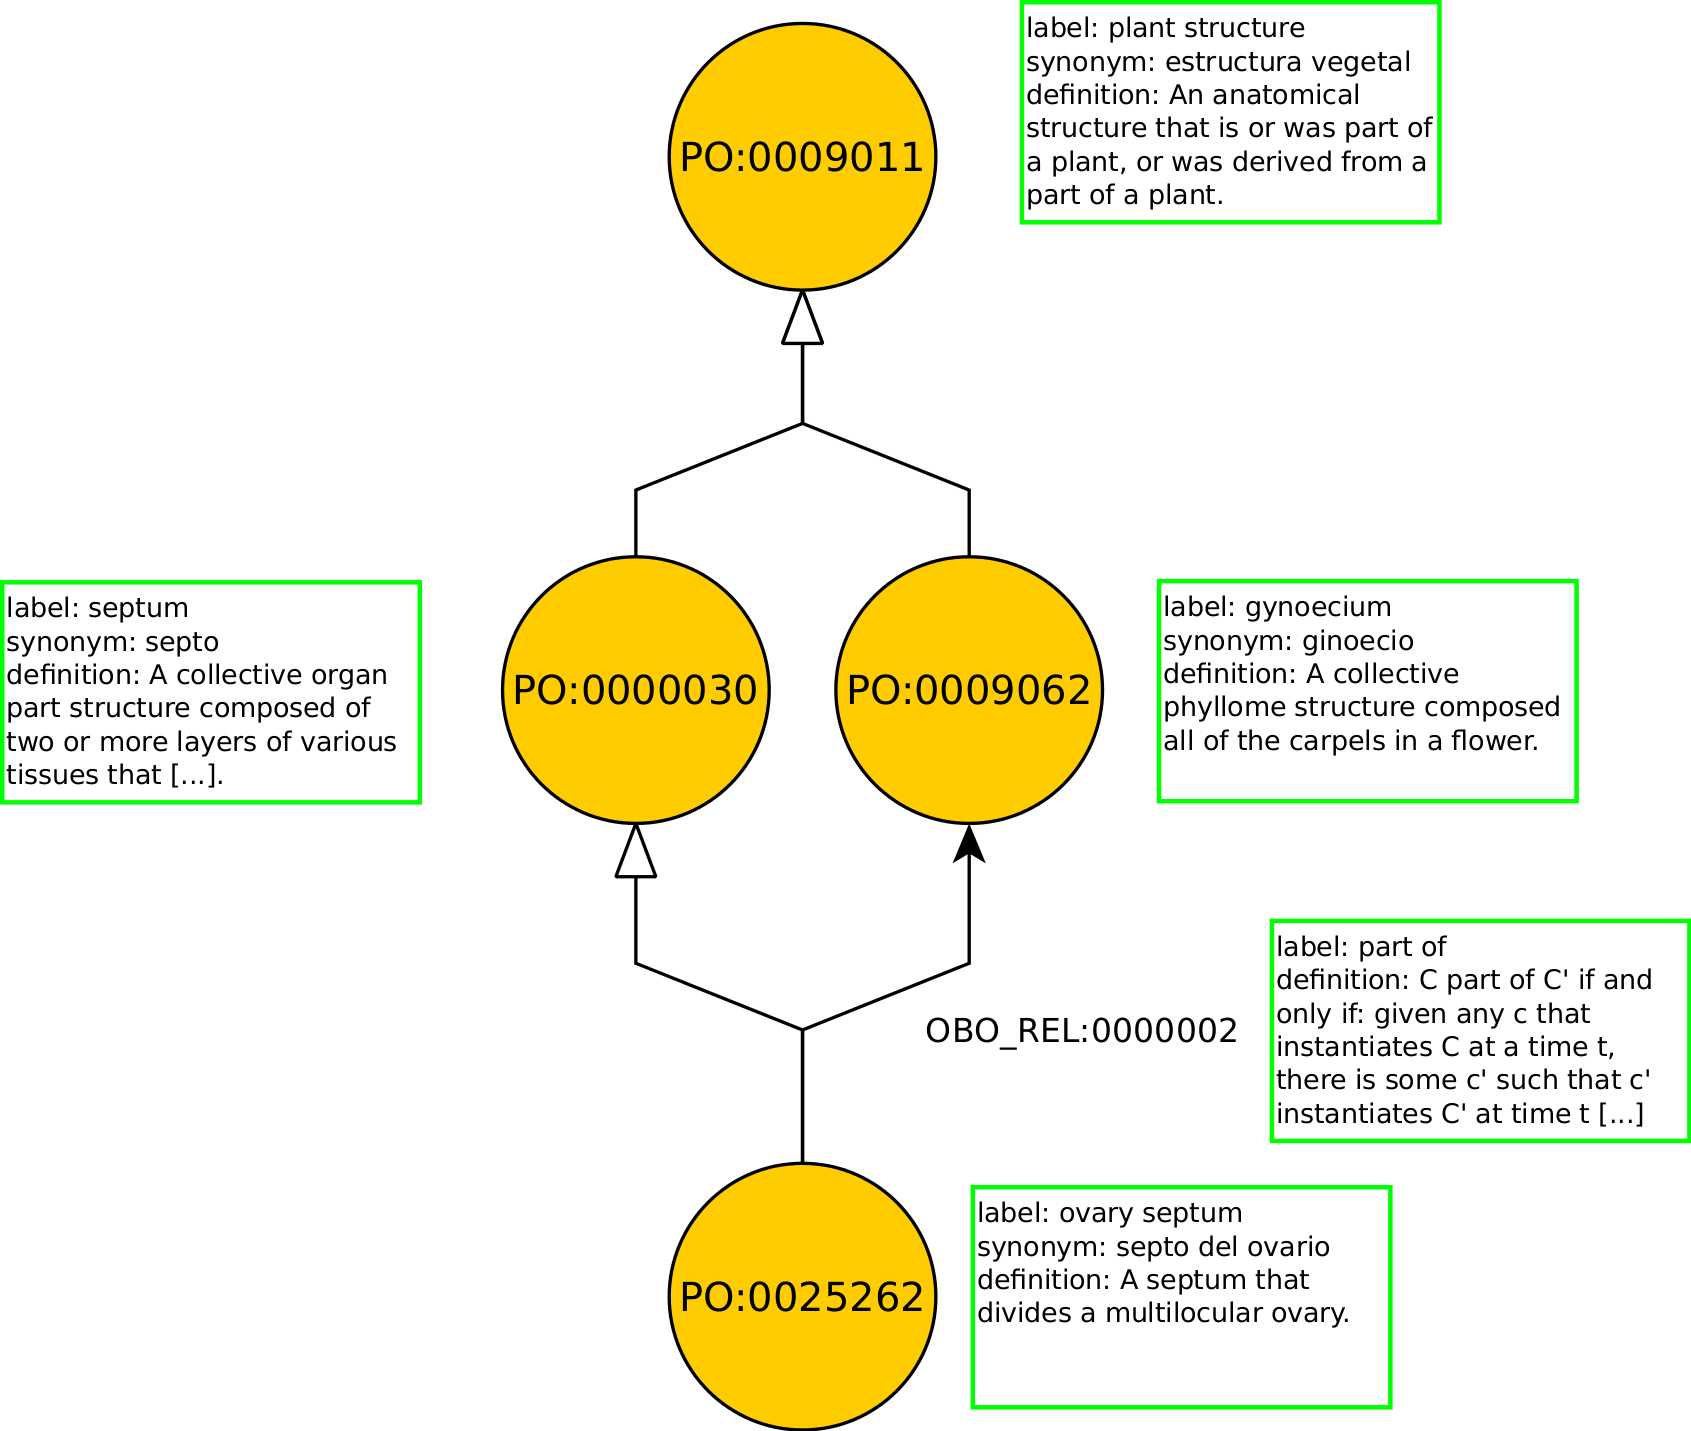
\includegraphics[height=.8\textheight]{plant-ontology-sample.png}}
\end{frame}

\begin{frame}
  \frametitle{Relations as patterns: Quiz}
  \begin{itemize}
  \item {\em classes}
    \begin{enumerate}[a]
    \item represent kinds of things in the world
    \item represent ideas in people's heads
    \item represent words
    \end{enumerate}
    \pause
  \item {\em instances} of a class are individuals that
    \begin{enumerate}[a]
    \item satisfy the class intension
    \item satisfy the axioms used to specify the class
    \item are always concrete, material entities
    \end{enumerate}
    \pause
  \item {\em relations} between classes are
    \begin{enumerate}[a]
    \item interactions between instances of the class
    \item abbreviations of axioms that constrain two classes
    \item relations between ideas people have about the classes
    \end{enumerate}
    \pause
  \item {\em axioms} are
    \begin{enumerate}[a]
    \item specification of conditions that instances of classes must satisfy
    \item rules that can be executed to produce new knowledge
    \item statements that are considered to be true in a domain of knowledge
    \end{enumerate}
  \end{itemize}
\end{frame}

\begin{frame}
  \frametitle{How to measure similarity?}
  What properties do we want in a similarity measure?
  \begin{itemize}
  \item a function $sim: D \times D$ is a similarity on $D$ if, for
    all $x, y \in D$, the function $sim$ is:
    \pause
  \item non-negative: $sim(x,y) \geq 0$ for all $x, y$
    \pause
  \item symmetric: $sim(x,y) = sim(y,x)$
    \pause
  \item reflexive: $sim(x,x) = max_D$
    \pause
  \item $sim(x,x) > sim(x,y)$ if $x\not= y$
    \pause
  \item $sim$ is a {\em normalized} similarity measure if it has
    values in $[0,1]$
  \end{itemize}
\end{frame}

\begin{frame}
  \frametitle{How to measure similarity?}
  \begin{columns}
    \begin{column}{.6\textwidth}
      {\tiny
        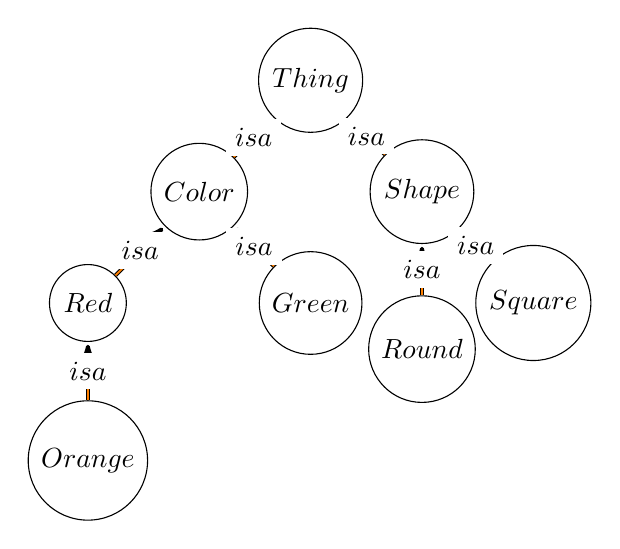
\begin{tikzpicture}[>=stealth',shorten >=1pt,node distance=2cm,on grid,initial/.style    ={}]
          \node[state]          (A)                        {$Thing$};
          \node[state]          (B) [below left =of A]    {$Color$};
          \node[state]          (C) [below right =of A]    {$Shape$};
          \node[state]          (D) [below left =of B]    {$Red$};
          \node[state]          (H) [below right =of B]    {$Green$};
          \node[state]          (E) [below  =of D]    {$Orange$};
          \node[state]          (F) [below =of C]    {$Round$};
          \node[state]          (G) [below right =of C]    {$Square$};
          \tikzset{mystyle/.style={->,double=orange}} 
          \tikzset{every node/.style={fill=white}} 
          \path (B)     edge [mystyle]    node   {$isa$} (A)
          (C)     edge [mystyle]    node   {$isa$} (A) 
          (D)     edge [mystyle]    node   {$isa$} (B)
          (H)     edge [mystyle]    node   {$isa$} (B)
          (E)     edge [mystyle]    node   {$isa$} (D)
          (F)     edge [mystyle]    node   {$isa$} (C)
          (G)     edge [mystyle]    node   {$isa$} (C);
          \tikzset{mystyle/.style={<->,double=orange}}   
          \tikzset{mystyle/.style={<->,relative=true,in=0,out=60,double=orange}}
        \end{tikzpicture}
      }
    \end{column}
    \begin{column}{.4\textwidth}
      \begin{itemize}
        \pause
      \item distance on shortest path (Rada {\em et al.}, 1989)
        \pause
      \item $dist_{Rada}(u,v) = sp(u, isa, v)$
        \pause
      \item $sim_{Rada}(u,v) = \frac{1}{dist_{Rada}(u,v) + 1}$
      \end{itemize}
    \end{column}
  \end{columns}
\end{frame}

\begin{frame}
  \frametitle{How to measure similarity?}
  \begin{columns}
    \begin{column}{.6\textwidth}
      {\tiny
        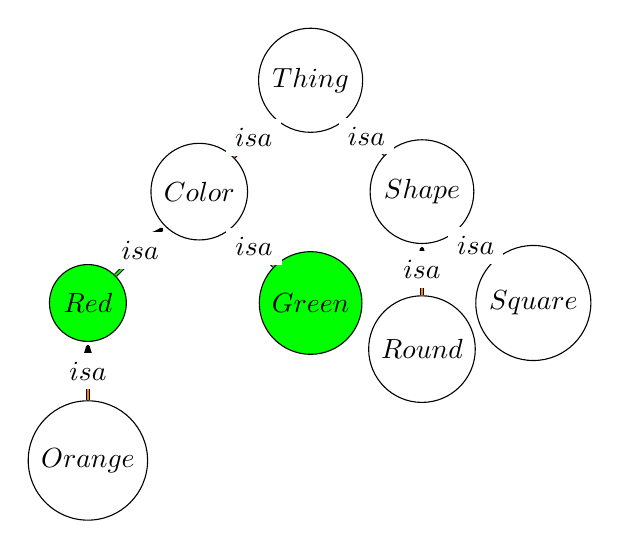
\begin{tikzpicture}[>=stealth',shorten >=1pt,node distance=2cm,on grid,initial/.style    ={}]
          \node[state]          (A)                        {$Thing$};
          \node[state]          (B) [below left =of A]    {$Color$};
          \node[state]          (C) [below right =of A]    {$Shape$};
          \node[state, fill=green]          (D) [below left =of B]    {$Red$};
          \node[state, fill=green]          (H) [below right =of B]    {$Green$};
          \node[state]          (E) [below  =of D]    {$Orange$};
          \node[state]          (F) [below =of C]    {$Round$};
          \node[state]          (G) [below right =of C]    {$Square$};
          \tikzset{mystyle/.style={->,double=orange}} 
          \tikzset{highlight/.style={->,double=green}} 
          \tikzset{every node/.style={fill=white}}
          \path (B)     edge [mystyle]    node   {$isa$} (A)
          (C)     edge [mystyle]    node   {$isa$} (A) 
          (D)     edge [highlight]    node   {$isa$} (B)
          (H)     edge [highlight]    node   {$isa$} (B)
          (E)     edge [mystyle]    node   {$isa$} (D)
          (F)     edge [mystyle]    node   {$isa$} (C)
          (G)     edge [mystyle]    node   {$isa$} (C);
          \tikzset{mystyle/.style={<->,double=orange}}   
          \tikzset{mystyle/.style={<->,relative=true,in=0,out=60,double=orange}}
        \end{tikzpicture}
      }
    \end{column}
    \begin{column}{.4\textwidth}
      \begin{itemize}
       \item distance on shortest path
       \item distance(green, red) = 2
       \item $sim_{Rada}(green, red) = \frac{1}{3}$
      \end{itemize}
    \end{column}
  \end{columns}
\end{frame}

\begin{frame}
  \frametitle{How to measure similarity?}
  \begin{columns}
    \begin{column}{.6\textwidth}
      {\tiny
        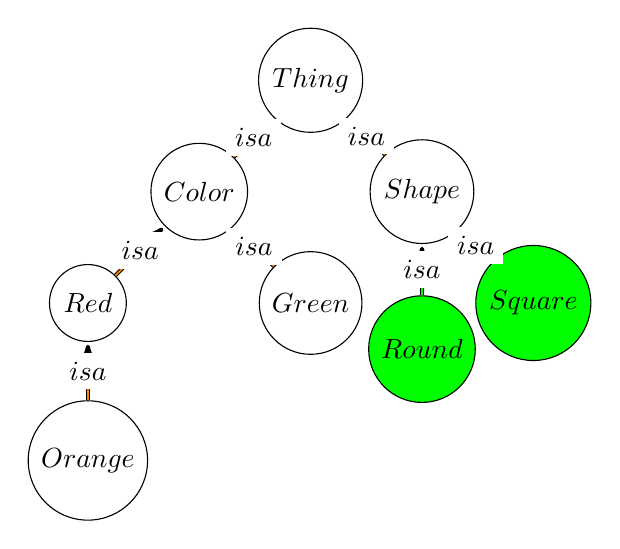
\begin{tikzpicture}[>=stealth',shorten >=1pt,node distance=2cm,on grid,initial/.style    ={}]
          \node[state]          (A)                        {$Thing$};
          \node[state]          (B) [below left =of A]    {$Color$};
          \node[state]          (C) [below right =of A]    {$Shape$};
          \node[state]          (D) [below left =of B]    {$Red$};
          \node[state]          (H) [below right =of B]    {$Green$};
          \node[state]          (E) [below  =of D]    {$Orange$};
          \node[state, fill=green]          (F) [below =of C]    {$Round$};
          \node[state, fill=green]          (G) [below right =of C]    {$Square$};
          \tikzset{mystyle/.style={->,double=orange}} 
          \tikzset{highlight/.style={->,double=green}} 
          \tikzset{every node/.style={fill=white}}
          \path (B)     edge [mystyle]    node   {$isa$} (A)
          (C)     edge [mystyle]    node   {$isa$} (A) 
          (D)     edge [mystyle]    node   {$isa$} (B)
          (H)     edge [mystyle]    node   {$isa$} (B)
          (E)     edge [mystyle]    node   {$isa$} (D)
          (F)     edge [highlight]    node   {$isa$} (C)
          (G)     edge [highlight]    node   {$isa$} (C);
          \tikzset{mystyle/.style={<->,double=orange}}   
          \tikzset{mystyle/.style={<->,relative=true,in=0,out=60,double=orange}}
        \end{tikzpicture}
      }
    \end{column}
    \begin{column}{.4\textwidth}
      \begin{itemize}
       \item distance on shortest path
       \item distance(square, round) = 2
       \item $sim_{Rada}(square, round) = \frac{1}{3}$
      \end{itemize}
    \end{column}
  \end{columns}
\end{frame}

\begin{frame}
  \frametitle{How to measure similarity?}
  \begin{columns}
    \begin{column}{.6\textwidth}
      {\tiny
        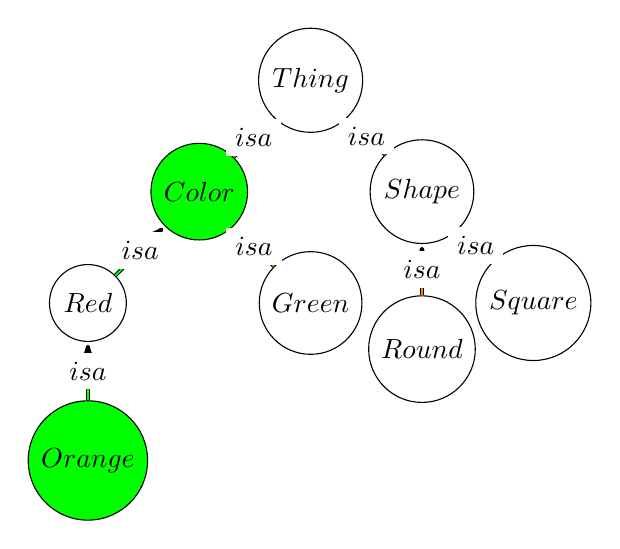
\begin{tikzpicture}[>=stealth',shorten >=1pt,node distance=2cm,on grid,initial/.style    ={}]
          \node[state]          (A)                        {$Thing$};
          \node[state, fill=green]          (B) [below left =of A]    {$Color$};
          \node[state]          (C) [below right =of A]    {$Shape$};
          \node[state]          (D) [below left =of B]    {$Red$};
          \node[state]          (H) [below right =of B]    {$Green$};
          \node[state, fill=green]          (E) [below  =of D]    {$Orange$};
          \node[state]          (F) [below =of C]    {$Round$};
          \node[state]          (G) [below right =of C]    {$Square$};
          \tikzset{mystyle/.style={->,double=orange}} 
          \tikzset{highlight/.style={->,double=green}} 
          \tikzset{every node/.style={fill=white}}
          \path (B)     edge [mystyle]    node   {$isa$} (A)
          (C)     edge [mystyle]    node   {$isa$} (A) 
          (D)     edge [highlight]    node   {$isa$} (B)
          (H)     edge [mystyle]    node   {$isa$} (B)
          (E)     edge [highlight]    node   {$isa$} (D)
          (F)     edge [mystyle]    node   {$isa$} (C)
          (G)     edge [mystyle]    node   {$isa$} (C);
          \tikzset{mystyle/.style={<->,double=orange}}   
          \tikzset{mystyle/.style={<->,relative=true,in=0,out=60,double=orange}}
        \end{tikzpicture}
      }
    \end{column}
    \begin{column}{.4\textwidth}
      \begin{itemize}
       \item distance on shortest path
       \item distance(orange, color) = 2
       \item $sim_{Rada}(orange, color) = \frac{1}{3}$
      \end{itemize}
    \end{column}
  \end{columns}
\end{frame}

\begin{frame}
  \frametitle{How to measure similarity?}
  \begin{itemize}
  \item shortest path is not always intuitive
    \pause
  \item we need a way to determine {\em specificity} of a class
    \begin{itemize}
    \item number of ancestors
    \item number of children
    \item information content
    \end{itemize}
    \pause
  \item {\em density} of a branch in the ontology
    \begin{itemize}
    \item number of siblings
    \item information content
    \end{itemize}
    \pause
  \item account for different edge types
    \begin{itemize}
    \item non-uniform edge weighting
    \end{itemize}
  \end{itemize}
\end{frame}

\begin{frame}
  \frametitle{How to measure similarity}
  \begin{itemize}
  \item term specificity measure $\sigma: C \mapsto \mathbb{R}$:
    \begin{itemize}
    \item $x \sqsubseteq y \rightarrow \sigma(x) \geq \sigma(y)$
    \end{itemize}
    \pause
  \item intrinsic:
    \begin{itemize}
    \item $\sigma(x) = depth(x)$
    \item $\sigma(x) = f(A(x))$ (for ancestors $A(x)$)
    \item $\sigma(x) = f(D(x))$ (for descendants $D(x)$)
    \item many more, e.g., Zhou et al.: $\sigma(x) = k \cdot \Big( 1-\frac{\log
        |D(x)|}{\log |C|} \Big) + (1-k) \frac{\log depth(x)}{\log
        depth(G_T)} $
    \end{itemize}
    \pause
  \item extrinsic:
    \begin{itemize}
    \item $\sigma(x)$ defined as a function of instances (or annotations) $I$
      \begin{itemize}
      \item note: the number of instances monotonically decreases with
        increasing depth in taxonomies
      \end{itemize}
    \item Resnik 1995: $eIC_{Resnik}(x) = -\log p(x)$ (with $p(x) =
      \frac{|I(x)|}{|I|}$)
      \begin{itemize}
      \item in biology, the most popular specificity measure when
        annotations are present
      \end{itemize}
    \end{itemize}
  \end{itemize}
\end{frame}

\begin{frame}
  \frametitle{How to measure similarity?}
  \begin{columns}
    \begin{column}{.6\textwidth}
      {\tiny
        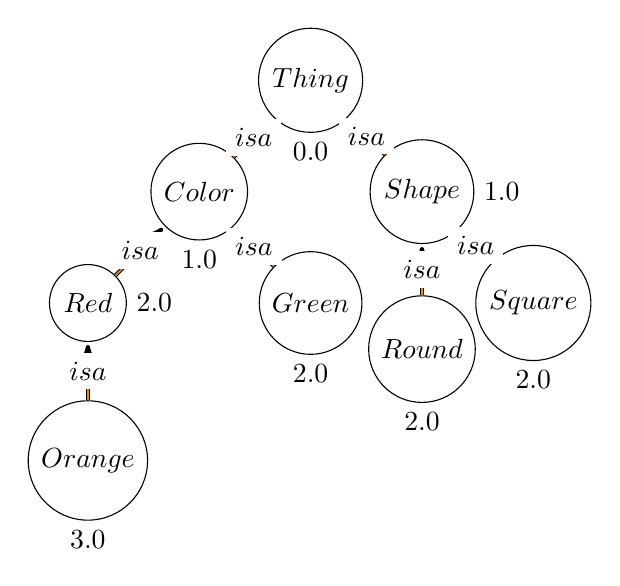
\begin{tikzpicture}[>=stealth',shorten >=1pt,node distance=2cm,on grid,initial/.style    ={}]
          \node[state,label=below:$0.0$]          (A)                        {$Thing$};
          \node[state,label=below:$1.0$]          (B) [below left =of A]    {$Color$};
          \node[state,label=right:$1.0$]          (C) [below right =of A]    {$Shape$};
          \node[state,label=right:$2.0$]          (D) [below left =of B]    {$Red$};
          \node[state,label=below:$2.0$]          (H) [below right =of B]    {$Green$};
          \node[state,label=below:$3.0$]          (E) [below  =of D]    {$Orange$};
          \node[state,label=below:$2.0$]          (F) [below =of C]    {$Round$};
          \node[state,label=below:$2.0$]          (G) [below right =of C]    {$Square$};
          \tikzset{mystyle/.style={->,double=orange}} 
          \tikzset{highlight/.style={->,double=green}} 
          \tikzset{every node/.style={fill=white}}
          \path (B)     edge [mystyle]    node   {$isa$} (A)
          (C)     edge [mystyle]    node   {$isa$} (A) 
          (D)     edge [mystyle]    node   {$isa$} (B)
          (H)     edge [mystyle]    node   {$isa$} (B)
          (E)     edge [mystyle]    node   {$isa$} (D)
          (F)     edge [mystyle]    node   {$isa$} (C)
          (G)     edge [mystyle]    node   {$isa$} (C);
          \tikzset{mystyle/.style={<->,double=orange}}   
          \tikzset{mystyle/.style={<->,relative=true,in=0,out=60,double=orange}}
        \end{tikzpicture}
      }
    \end{column}
    \begin{column}{.4\textwidth}
      \begin{itemize}
      \item Resnik 1995: similarity between $x$ and $y$ is the
        information content of the {\em most informative common
          ancestor}
      \end{itemize}
    \end{column}
  \end{columns}
\end{frame}

\begin{frame}
  \frametitle{How to measure similarity?}
  \begin{columns}
    \begin{column}{.6\textwidth}
      {\tiny
        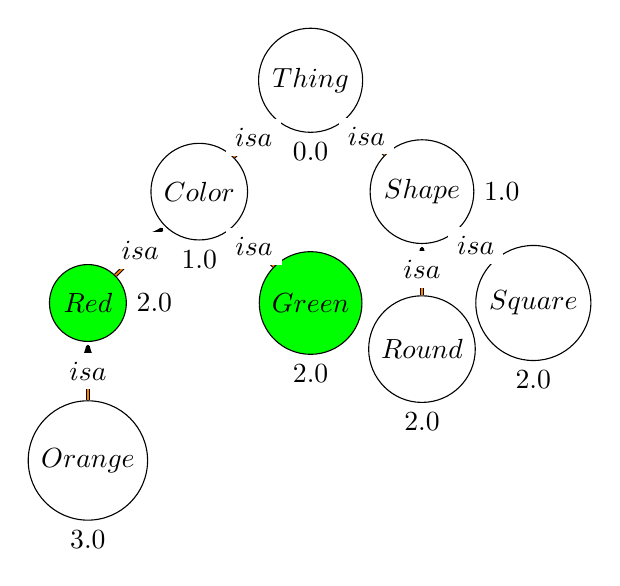
\begin{tikzpicture}[>=stealth',shorten >=1pt,node distance=2cm,on grid,initial/.style    ={}]
          \node[state,label=below:$0.0$]          (A)                        {$Thing$};
          \node[state,label=below:$1.0$]          (B) [below left =of A]    {$Color$};
          \node[state,label=right:$1.0$]          (C) [below right =of A]    {$Shape$};
          \node[state,fill=green,label=right:$2.0$]          (D) [below left =of B]    {$Red$};
          \node[state,fill=green,label=below:$2.0$]          (H) [below right =of B]    {$Green$};
          \node[state,label=below:$3.0$]          (E) [below  =of D]    {$Orange$};
          \node[state,label=below:$2.0$]          (F) [below =of C]    {$Round$};
          \node[state,label=below:$2.0$]          (G) [below right =of C]    {$Square$};
          \tikzset{mystyle/.style={->,double=orange}} 
          \tikzset{highlight/.style={->,double=green}} 
          \tikzset{every node/.style={fill=white}}
          \path (B)     edge [mystyle]    node   {$isa$} (A)
          (C)     edge [mystyle]    node   {$isa$} (A) 
          (D)     edge [mystyle]    node   {$isa$} (B)
          (H)     edge [mystyle]    node   {$isa$} (B)
          (E)     edge [mystyle]    node   {$isa$} (D)
          (F)     edge [mystyle]    node   {$isa$} (C)
          (G)     edge [mystyle]    node   {$isa$} (C);
          \tikzset{mystyle/.style={<->,double=orange}}   
          \tikzset{mystyle/.style={<->,relative=true,in=0,out=60,double=orange}}
        \end{tikzpicture}
      }
    \end{column}
    \begin{column}{.4\textwidth}
      \begin{itemize}
      \item Resnik 1995: similarity between $x$ and $y$ is the
        information content of the {\em most informative common
          ancestor}
      \end{itemize}
    \end{column}
  \end{columns}
\end{frame}

\begin{frame}
  \frametitle{How to measure similarity?}
  \begin{columns}
    \begin{column}{.6\textwidth}
      {\tiny
        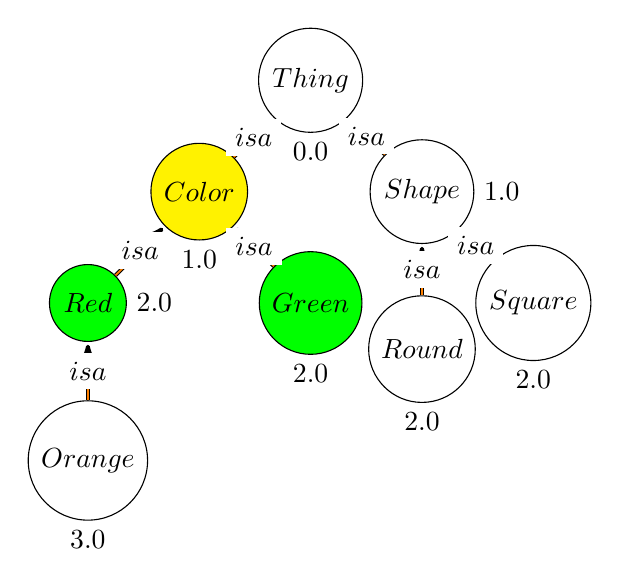
\begin{tikzpicture}[>=stealth',shorten >=1pt,node distance=2cm,on grid,initial/.style    ={}]
          \node[state,label=below:$0.0$]          (A)                        {$Thing$};
          \node[state,fill=yellow,label=below:$1.0$]          (B) [below left =of A]    {$Color$};
          \node[state,label=right:$1.0$]          (C) [below right =of A]    {$Shape$};
          \node[state,fill=green,label=right:$2.0$]          (D) [below left =of B]    {$Red$};
          \node[state,fill=green,label=below:$2.0$]          (H) [below right =of B]    {$Green$};
          \node[state,label=below:$3.0$]          (E) [below  =of D]    {$Orange$};
          \node[state,label=below:$2.0$]          (F) [below =of C]    {$Round$};
          \node[state,label=below:$2.0$]          (G) [below right =of C]    {$Square$};
          \tikzset{mystyle/.style={->,double=orange}} 
          \tikzset{highlight/.style={->,double=green}} 
          \tikzset{every node/.style={fill=white}}
          \path (B)     edge [mystyle]    node   {$isa$} (A)
          (C)     edge [mystyle]    node   {$isa$} (A) 
          (D)     edge [mystyle]    node   {$isa$} (B)
          (H)     edge [mystyle]    node   {$isa$} (B)
          (E)     edge [mystyle]    node   {$isa$} (D)
          (F)     edge [mystyle]    node   {$isa$} (C)
          (G)     edge [mystyle]    node   {$isa$} (C);
          \tikzset{mystyle/.style={<->,double=orange}}   
          \tikzset{mystyle/.style={<->,relative=true,in=0,out=60,double=orange}}
        \end{tikzpicture}
      }
    \end{column}
    \begin{column}{.4\textwidth}
      \begin{itemize}
      \item Resnik 1995: similarity between $x$ and $y$ is the
        information content of the {\em most informative common
          ancestor}
      \end{itemize}
    \end{column}
  \end{columns}
\end{frame}

\begin{frame}
  \frametitle{How to measure similarity?}
  \begin{columns}
    \begin{column}{.6\textwidth}
      {\tiny
        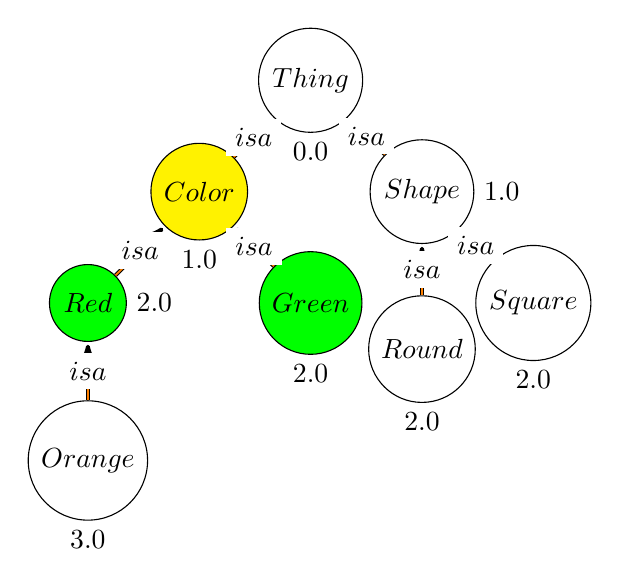
\begin{tikzpicture}[>=stealth',shorten >=1pt,node distance=2cm,on grid,initial/.style    ={}]
          \node[state,label=below:$0.0$]          (A)                        {$Thing$};
          \node[state,fill=yellow,label=below:$1.0$]          (B) [below left =of A]    {$Color$};
          \node[state,label=right:$1.0$]          (C) [below right =of A]    {$Shape$};
          \node[state,fill=green,label=right:$2.0$]          (D) [below left =of B]    {$Red$};
          \node[state,fill=green,label=below:$2.0$]          (H) [below right =of B]    {$Green$};
          \node[state,label=below:$3.0$]          (E) [below  =of D]    {$Orange$};
          \node[state,label=below:$2.0$]          (F) [below =of C]    {$Round$};
          \node[state,label=below:$2.0$]          (G) [below right =of C]    {$Square$};
          \tikzset{mystyle/.style={->,double=orange}} 
          \tikzset{highlight/.style={->,double=green}} 
          \tikzset{every node/.style={fill=white}}
          \path (B)     edge [mystyle]    node   {$isa$} (A)
          (C)     edge [mystyle]    node   {$isa$} (A) 
          (D)     edge [mystyle]    node   {$isa$} (B)
          (H)     edge [mystyle]    node   {$isa$} (B)
          (E)     edge [mystyle]    node   {$isa$} (D)
          (F)     edge [mystyle]    node   {$isa$} (C)
          (G)     edge [mystyle]    node   {$isa$} (C);
          \tikzset{mystyle/.style={<->,double=orange}}   
          \tikzset{mystyle/.style={<->,relative=true,in=0,out=60,double=orange}}
        \end{tikzpicture}
      }
    \end{column}
    \begin{column}{.4\textwidth}
      \begin{itemize}
      \item Resnik 1995: similarity between $x$ and $y$ is the
        information content of the {\em most informative common
          ancestor}
        \item $sim_{Resnik}(Green, Red) = 1.0$
      \end{itemize}
    \end{column}
  \end{columns}
\end{frame}

\begin{frame}
  \frametitle{How to measure similarity?}
  \begin{columns}
    \begin{column}{.6\textwidth}
      {\tiny
        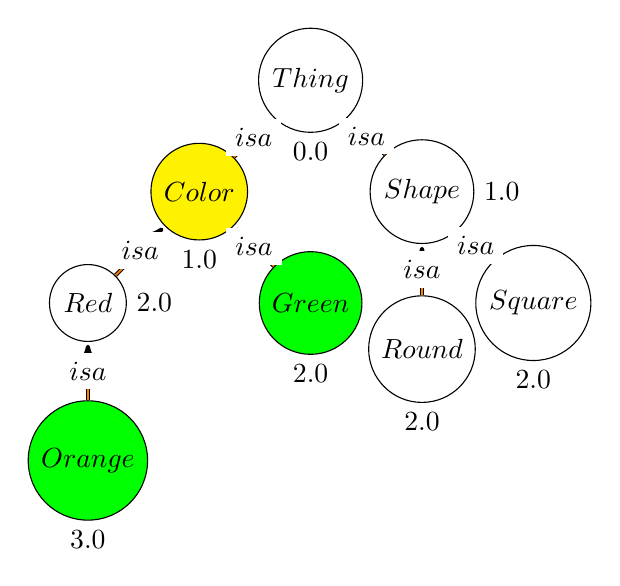
\begin{tikzpicture}[>=stealth',shorten >=1pt,node distance=2cm,on grid,initial/.style    ={}]
          \node[state,label=below:$0.0$]          (A)                        {$Thing$};
          \node[state,fill=yellow,label=below:$1.0$]          (B) [below left =of A]    {$Color$};
          \node[state,label=right:$1.0$]          (C) [below right =of A]    {$Shape$};
          \node[state,label=right:$2.0$]          (D) [below left =of B]    {$Red$};
          \node[state,fill=green,label=below:$2.0$]          (H) [below right =of B]    {$Green$};
          \node[state,fill=green,label=below:$3.0$]          (E) [below  =of D]    {$Orange$};
          \node[state,label=below:$2.0$]          (F) [below =of C]    {$Round$};
          \node[state,label=below:$2.0$]          (G) [below right =of C]    {$Square$};
          \tikzset{mystyle/.style={->,double=orange}} 
          \tikzset{highlight/.style={->,double=green}} 
          \tikzset{every node/.style={fill=white}}
          \path (B)     edge [mystyle]    node   {$isa$} (A)
          (C)     edge [mystyle]    node   {$isa$} (A) 
          (D)     edge [mystyle]    node   {$isa$} (B)
          (H)     edge [mystyle]    node   {$isa$} (B)
          (E)     edge [mystyle]    node   {$isa$} (D)
          (F)     edge [mystyle]    node   {$isa$} (C)
          (G)     edge [mystyle]    node   {$isa$} (C);
          \tikzset{mystyle/.style={<->,double=orange}}   
          \tikzset{mystyle/.style={<->,relative=true,in=0,out=60,double=orange}}
        \end{tikzpicture}
      }
    \end{column}
    \begin{column}{.4\textwidth}
      \begin{itemize}
      \item Resnik 1995: similarity between $x$ and $y$ is the
        information content of the {\em most informative common
          ancestor}
        \item $sim_{Resnik}(Green, Orange) = 1.0$
      \end{itemize}
    \end{column}
  \end{columns}
\end{frame}

\begin{frame}
  \frametitle{How to measure similarity?}
  \begin{columns}
    \begin{column}{.6\textwidth}
      {\tiny
        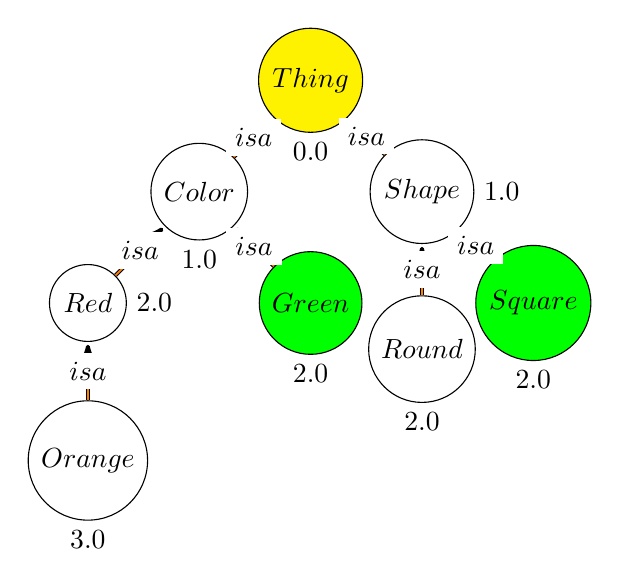
\begin{tikzpicture}[>=stealth',shorten >=1pt,node distance=2cm,on grid,initial/.style    ={}]
          \node[state,fill=yellow,label=below:$0.0$]          (A)                        {$Thing$};
          \node[state,label=below:$1.0$]          (B) [below left =of A]    {$Color$};
          \node[state,label=right:$1.0$]          (C) [below right =of A]    {$Shape$};
          \node[state,label=right:$2.0$]          (D) [below left =of B]    {$Red$};
          \node[state,fill=green,label=below:$2.0$]          (H) [below right =of B]    {$Green$};
          \node[state,label=below:$3.0$]          (E) [below  =of D]    {$Orange$};
          \node[state,label=below:$2.0$]          (F) [below =of C]    {$Round$};
          \node[state,fill=green,label=below:$2.0$]          (G) [below right =of C]    {$Square$};
          \tikzset{mystyle/.style={->,double=orange}} 
          \tikzset{highlight/.style={->,double=green}} 
          \tikzset{every node/.style={fill=white}}
          \path (B)     edge [mystyle]    node   {$isa$} (A)
          (C)     edge [mystyle]    node   {$isa$} (A) 
          (D)     edge [mystyle]    node   {$isa$} (B)
          (H)     edge [mystyle]    node   {$isa$} (B)
          (E)     edge [mystyle]    node   {$isa$} (D)
          (F)     edge [mystyle]    node   {$isa$} (C)
          (G)     edge [mystyle]    node   {$isa$} (C);
          \tikzset{mystyle/.style={<->,double=orange}}   
          \tikzset{mystyle/.style={<->,relative=true,in=0,out=60,double=orange}}
        \end{tikzpicture}
      }
    \end{column}
    \begin{column}{.4\textwidth}
      \begin{itemize}
      \item Resnik 1995: similarity between $x$ and $y$ is the
        information content of the {\em most informative common
          ancestor}
        \item $sim_{Resnik}(Square, Orange) = 0.0$
      \end{itemize}
    \end{column}
  \end{columns}
\end{frame}

\begin{frame}
  \frametitle{How to measure similarity?}
  \begin{itemize}
  \item (Red, Green) and (Orange, Green) have the same similarity
  \item need to incorporate the specificity of the compared classes
  \end{itemize}
\end{frame}

\begin{frame}
  \frametitle{How to measure similarity?}
  \begin{columns}
    \begin{column}{.6\textwidth}
      {\tiny
        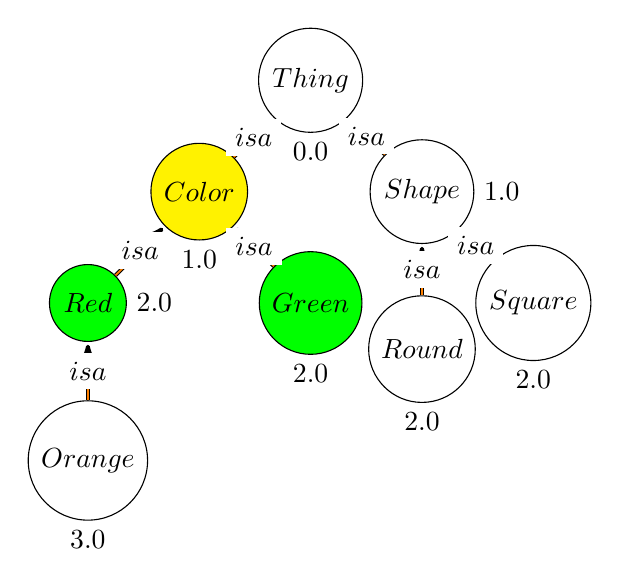
\begin{tikzpicture}[>=stealth',shorten >=1pt,node distance=2cm,on grid,initial/.style    ={}]
          \node[state,label=below:$0.0$]          (A)                        {$Thing$};
          \node[state,fill=yellow,label=below:$1.0$]          (B) [below left =of A]    {$Color$};
          \node[state,label=right:$1.0$]          (C) [below right =of A]    {$Shape$};
          \node[state,fill=green,label=right:$2.0$]          (D) [below left =of B]    {$Red$};
          \node[state,fill=green,label=below:$2.0$]          (H) [below right =of B]    {$Green$};
          \node[state,label=below:$3.0$]          (E) [below  =of D]    {$Orange$};
          \node[state,label=below:$2.0$]          (F) [below =of C]    {$Round$};
          \node[state,label=below:$2.0$]          (G) [below right =of C]    {$Square$};
          \tikzset{mystyle/.style={->,double=orange}} 
          \tikzset{highlight/.style={->,double=green}} 
          \tikzset{every node/.style={fill=white}}
          \path (B)     edge [mystyle]    node   {$isa$} (A)
          (C)     edge [mystyle]    node   {$isa$} (A) 
          (D)     edge [mystyle]    node   {$isa$} (B)
          (H)     edge [mystyle]    node   {$isa$} (B)
          (E)     edge [mystyle]    node   {$isa$} (D)
          (F)     edge [mystyle]    node   {$isa$} (C)
          (G)     edge [mystyle]    node   {$isa$} (C);
          \tikzset{mystyle/.style={<->,double=orange}}   
          \tikzset{mystyle/.style={<->,relative=true,in=0,out=60,double=orange}}
        \end{tikzpicture}
      }
    \end{column}
    \begin{column}{.4\textwidth}
      \begin{itemize}
      \item Lin 1998: $sim_{Lin}(x,y) = \frac{2\cdot
          IC(MICA(x,y))}{IC(x) + IC(y)}$
        \pause
      \item $sim_{Lin}(Green, Red) = 0.5$
      \end{itemize}
    \end{column}
  \end{columns}
\end{frame}

\begin{frame}
  \frametitle{How to measure similarity?}
  \begin{columns}
    \begin{column}{.6\textwidth}
      {\tiny
        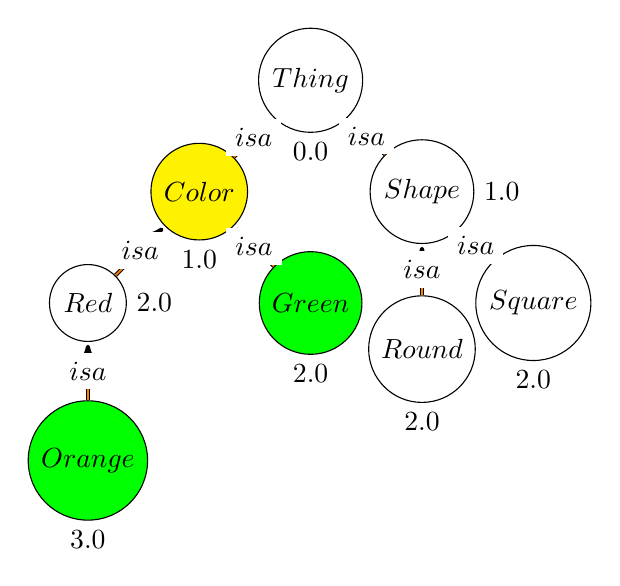
\begin{tikzpicture}[>=stealth',shorten >=1pt,node distance=2cm,on grid,initial/.style    ={}]
          \node[state,label=below:$0.0$]          (A)                        {$Thing$};
          \node[state,fill=yellow,label=below:$1.0$]          (B) [below left =of A]    {$Color$};
          \node[state,label=right:$1.0$]          (C) [below right =of A]    {$Shape$};
          \node[state,label=right:$2.0$]          (D) [below left =of B]    {$Red$};
          \node[state,fill=green,label=below:$2.0$]          (H) [below right =of B]    {$Green$};
          \node[state,fill=green,label=below:$3.0$]          (E) [below  =of D]    {$Orange$};
          \node[state,label=below:$2.0$]          (F) [below =of C]    {$Round$};
          \node[state,label=below:$2.0$]          (G) [below right =of C]    {$Square$};
          \tikzset{mystyle/.style={->,double=orange}} 
          \tikzset{highlight/.style={->,double=green}} 
          \tikzset{every node/.style={fill=white}}
          \path (B)     edge [mystyle]    node   {$isa$} (A)
          (C)     edge [mystyle]    node   {$isa$} (A) 
          (D)     edge [mystyle]    node   {$isa$} (B)
          (H)     edge [mystyle]    node   {$isa$} (B)
          (E)     edge [mystyle]    node   {$isa$} (D)
          (F)     edge [mystyle]    node   {$isa$} (C)
          (G)     edge [mystyle]    node   {$isa$} (C);
          \tikzset{mystyle/.style={<->,double=orange}}   
          \tikzset{mystyle/.style={<->,relative=true,in=0,out=60,double=orange}}
        \end{tikzpicture}
      }
    \end{column}
    \begin{column}{.4\textwidth}
      \begin{itemize}
      \item Lin 1998: $sim_{Lin}(x,y) = \frac{2\cdot
          IC(MICA(x,y))}{IC(x) + IC(y)}$
      \item $sim_{Lin}(Green, Orange) = 0.4$
      \end{itemize}
    \end{column}
  \end{columns}
\end{frame}

\begin{frame}
  \frametitle{How to measure similarity?}
  \begin{itemize}
  \item many(!) others:
    \begin{itemize}
    \item Jiang \& Conrath 1997
    \item Mazandu \& Mulder 2013
    \item Schlicker et al. 2009
    \item ...
  \end{itemize}
  \end{itemize}
\end{frame}

\begin{frame}
  \frametitle{How to measure similarity?}
  \begin{itemize}
  \item we only looked at comparing pairs of classes
  \item mostly, we want to compare {\em sets} of classes
    \begin{itemize}
    \item set of GO annotations
    \item set of signs and symptoms
    \item set of phenotypes
    \end{itemize}
  \item two approaches:
    \begin{itemize}
    \item compare each class individually, then merge
    \item directly set-based similarity measures
    \end{itemize}
  \end{itemize}
\end{frame}

\begin{frame}
  \frametitle{How to measure similarity?}
  \begin{columns}
    \begin{column}{.6\textwidth}
      {\tiny
        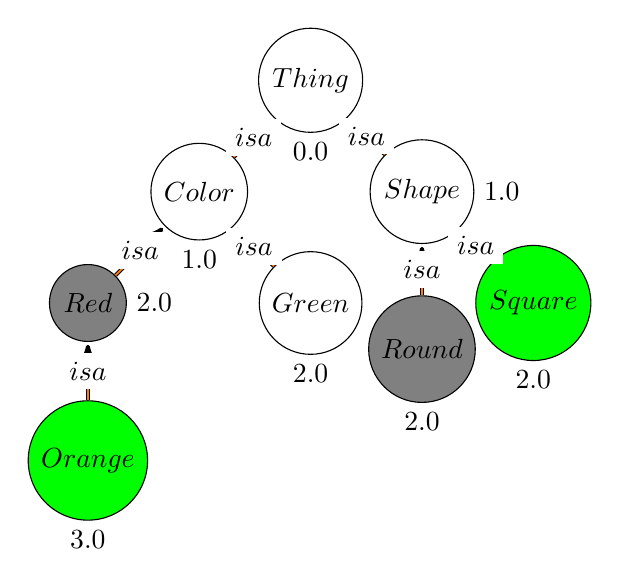
\begin{tikzpicture}[>=stealth',shorten >=1pt,node distance=2cm,on grid,initial/.style    ={}]
          \node[state,label=below:$0.0$]          (A)                        {$Thing$};
          \node[state,label=below:$1.0$]          (B) [below left =of A]    {$Color$};
          \node[state,label=right:$1.0$]          (C) [below right =of A]    {$Shape$};
          \node[state,fill=gray,label=right:$2.0$]          (D) [below left =of B]    {$Red$};
          \node[state,label=below:$2.0$]          (H) [below right =of B]    {$Green$};
          \node[state,fill=green,label=below:$3.0$]          (E) [below  =of D]    {$Orange$};
          \node[state,fill=gray,label=below:$2.0$]          (F) [below =of C]    {$Round$};
          \node[state,fill=green,label=below:$2.0$]          (G) [below right =of C]    {$Square$};
          \tikzset{mystyle/.style={->,double=orange}} 
          \tikzset{highlight/.style={->,double=green}} 
          \tikzset{every node/.style={fill=white}}
          \path (B)     edge [mystyle]    node   {$isa$} (A)
          (C)     edge [mystyle]    node   {$isa$} (A) 
          (D)     edge [mystyle]    node   {$isa$} (B)
          (H)     edge [mystyle]    node   {$isa$} (B)
          (E)     edge [mystyle]    node   {$isa$} (D)
          (F)     edge [mystyle]    node   {$isa$} (C)
          (G)     edge [mystyle]    node   {$isa$} (C);
          \tikzset{mystyle/.style={<->,double=orange}}   
          \tikzset{mystyle/.style={<->,relative=true,in=0,out=60,double=orange}}
        \end{tikzpicture}
      }
    \end{column}
    \begin{column}{.4\textwidth}
      \begin{itemize}
      \item similarity between a square-and-orange thing and a
        round-and-red thing
        \pause
      \item Pesquita et al., 2007:
        $simGIC(X,Y) = \frac{\sum_{c \in A(X) \cap A(Y)}
          IC(c)}{\sum_{c \in A(X) \cup A(Y)} IC(c)}$
      \end{itemize}
    \end{column}
  \end{columns}
\end{frame}

\begin{frame}
  \frametitle{How to measure similarity?}
  \begin{columns}
    \begin{column}{.6\textwidth}
      {\tiny
        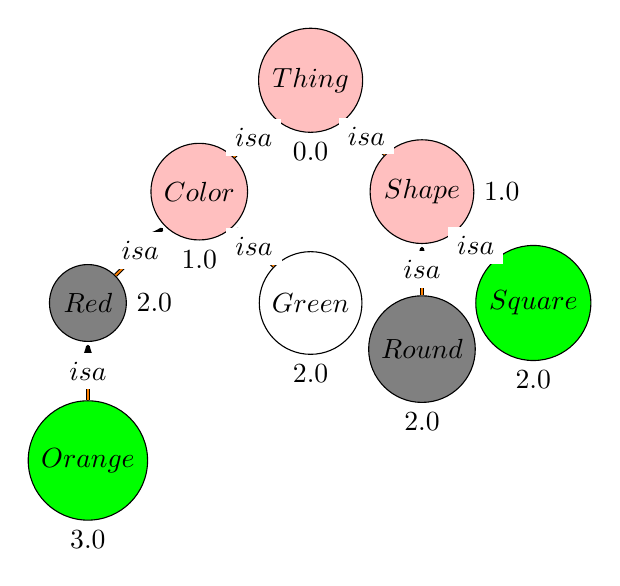
\begin{tikzpicture}[>=stealth',shorten >=1pt,node distance=2cm,on grid,initial/.style    ={}]
          \node[state,fill=pink,label=below:$0.0$]          (A)                        {$Thing$};
          \node[state,fill=pink,label=below:$1.0$]          (B) [below left =of A]    {$Color$};
          \node[state,fill=pink,label=right:$1.0$]          (C) [below right =of A]    {$Shape$};
          \node[state,fill=gray,label=right:$2.0$]          (D) [below left =of B]    {$Red$};
          \node[state,label=below:$2.0$]          (H) [below right =of B]    {$Green$};
          \node[state,fill=green,label=below:$3.0$]          (E) [below  =of D]    {$Orange$};
          \node[state,fill=gray,label=below:$2.0$]          (F) [below =of C]    {$Round$};
          \node[state,fill=green,label=below:$2.0$]          (G) [below right =of C]    {$Square$};
          \tikzset{mystyle/.style={->,double=orange}} 
          \tikzset{highlight/.style={->,double=green}} 
          \tikzset{every node/.style={fill=white}}
          \path (B)     edge [mystyle]    node   {$isa$} (A)
          (C)     edge [mystyle]    node   {$isa$} (A) 
          (D)     edge [mystyle]    node   {$isa$} (B)
          (H)     edge [mystyle]    node   {$isa$} (B)
          (E)     edge [mystyle]    node   {$isa$} (D)
          (F)     edge [mystyle]    node   {$isa$} (C)
          (G)     edge [mystyle]    node   {$isa$} (C);
          \tikzset{mystyle/.style={<->,double=orange}}   
          \tikzset{mystyle/.style={<->,relative=true,in=0,out=60,double=orange}}
        \end{tikzpicture}
      }
    \end{column}
    \begin{column}{.4\textwidth}
      \begin{itemize}
      \item similarity between a square-and-orange thing and a
        round-and-red thing
      \item Pesquita et al., 2007:
        $simGIC(X,Y) = \frac{\sum_{c \in A(X) \cap A(Y)}
          IC(c)}{\sum_{c \in A(X) \cup A(Y)} IC(c)}$
      \item $simGIC(so,rr) = \frac{2}{11}$
      \end{itemize}
    \end{column}
  \end{columns}
\end{frame}

\begin{frame}
  \frametitle{How to measure similarity?}
  \begin{itemize}
  \item alternatively: use different merging strategies
  \item common: average, maximum, {\bf best-matching average}
    \begin{itemize}
    \item Average: $sim_A(X,Y) = \frac{\sum_{x\in X} \sum_{y \in Y} sim(x,y)}{|X| \times |Y|}$
    \item Max average: $sim_{MA}(X,Y) = \frac{1}{|X|} \sum_{x\in X} \max_{y \in Y} sim(x,y)$
    \item Best match average: $sim_{BMA}(X,Y) = \frac{sim_{MA}(X,Y) + sim_{MA}(Y,X)}{2}$
    \end{itemize}
  \end{itemize}
\end{frame}

\begin{frame}
  \frametitle{How to measure similarity?}
  \begin{itemize}
  \item Semantic Measures Library:
    \begin{itemize}
    \item comprehensive Java library
    \item \url{http://www.semantic-measures-library.org/}
    \end{itemize}
  \item R packages: GOSim, GOSemSim, HPOSim, LSAfun,
    ontologySimilarity,...
  \item Python: sematch, fastsemsim (GO only)
  \end{itemize}
\end{frame}

\begin{frame}
  \frametitle{How to measure similarity?}
  \centerline{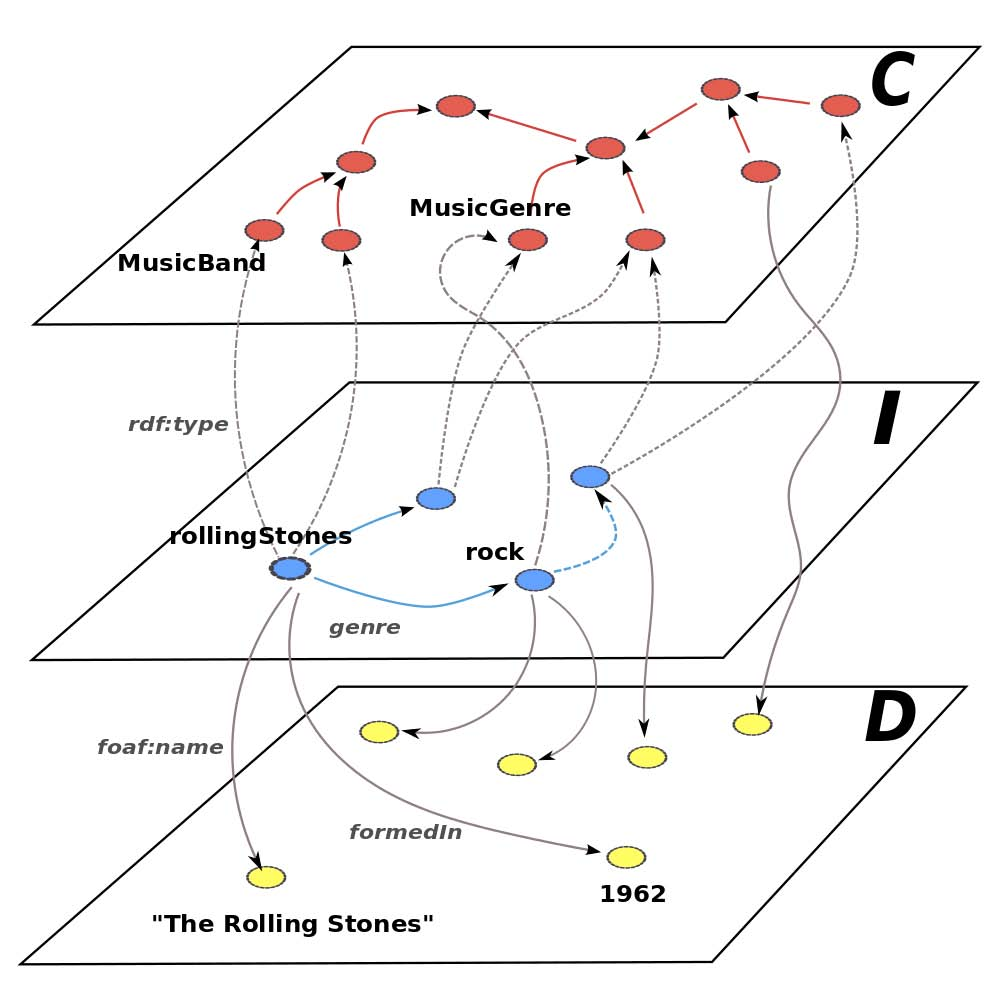
\includegraphics[height=.8\textheight]{instances.png}}
  {\tiny From Harispe et al., Semantic Similarity From Natural
    Language And Ontology Analysis, 2015.}
\end{frame}

\begin{frame}
  \frametitle{How to measure similarity?}
  \begin{itemize}
  \item Shortest Path
    \begin{itemize}
    \item applicable to arbitrary knowledge graphs
    \item does not capture similarity well over all edge types, e.g.,
      {\em disjointWith}, {\em differentFrom}, {\em opposite-of}, etc.
    \end{itemize}
  \item Random Walk
    \begin{itemize}
    \item with or without restart
    \item iterated
    \item does not consider edge labels $\Rightarrow$ captures only
      adjacency of nodes
    \item scores whole graph with {\em probability} of being in a
      state
    \item can take multiple seed nodes
      \begin{itemize}
      \item widely used to find disease genes
      \end{itemize}
    \end{itemize}
  \end{itemize}
\end{frame}

\begin{frame}
  \frametitle{How to measure similarity?}
  \begin{itemize}
  \item feature learning on knowledge graph
    \pause
  \item e.g., iterated, edge-labeled random walk
    \begin{itemize}
    \item over instances and classes
    \item walks form {\em sentences}
    \item sentences form a {\em corpus}
    \item feature learning on corpus through Word2Vec (or factorization
      of co-occurrence matrix)
    \item RDF2Vec:
      \url{http://data.dws.informatik.uni-mannheim.de/rdf2vec/}
      \begin{itemize}
      \item with support for reasoning:
        \url{https://github.com/bio-ontology-research-group/walking-rdf-and-owl}
      \end{itemize}
    \end{itemize}
    \pause
  \item Translational knowledge graph embeddings: TransE, TransR, TransE, HolE, etc.
    \begin{itemize}
    \item analogy-based
    \item \url{https://github.com/thunlp/KB2E}
    \end{itemize}
    \pause
  \item generates (dense) feature vectors for nodes (classes,
    instances) and relations
  \end{itemize}
\end{frame}

\begin{frame}
  \frametitle{How to measure similarity?}
  \centerline{\includegraphics[width=\textwidth]{workflow.png}}
\end{frame}

\begin{frame}
  \frametitle{How to measure similarity?}
  \begin{itemize}
  \item vector-based similarity measure
  \item cosine similarity: $sim(X,Y) = \frac{\sum_{i=1}^n X_i
      Y_i}{\sqrt{\sum_{i=1}^n X_i^2} \sqrt{\sum_{i=1}^n Y_i^2}} $
    \begin{itemize}
    \item bounded between $[-1,1]$
    \end{itemize}
  \item Euclidean distance: $sim(X,Y) = \sqrt{\sum_{i=1}^n (X_i - Y_i)^2}$
    \begin{itemize}
    \item not bounded (and rarely used)
    \end{itemize}
  \end{itemize}
\end{frame}

\begin{frame}
  \frametitle{How to measure similarity?}
  \begin{itemize}
  \item many graph based semantic similarity measures for comparing
    two classes
  \item several set-based measures
    \begin{itemize}
    \item directly set-based
    \item merging pair-wise comparison
    \end{itemize}
  \item most useful when comparing instances/annotations
  \item other approaches consider relations between instances:
    \begin{itemize}
    \item path-based
    \item random-walk
    \end{itemize}
  \item very recent: knowledge graph embeddings
    \begin{itemize}
    \item and any vector-based similarity measure
    \end{itemize}
  \end{itemize}
\end{frame}

\begin{frame}
  \frametitle{How to measure similarity?}
  Recommended reading:
  \begin{itemize}
  \item recommended, comprehensive overview: Sebastian Harispe et
    al. Semantic Similarity from Natural Language and Ontology
    Analysis. Morgan \& Claypool Publishers, 2015
  \item Catia Pesquita et al. Semantic Similarity in Biomedical
    Ontologies. PLoS CB, 2009.
  \item Maximilian Nickel et al. A Review of Relational Machine
    Learning for Knowledge Graphs, Proceedings of the IEEE, 2016.
  \end{itemize}
\end{frame}

\begin{frame}
  \frametitle{How to measure similarity: Quiz}
  \begin{itemize}
  \item How many semantic similarity measures are there?
    \begin{enumerate}[a]
    \item One (and it is called The Semantic Similarity Measure)
    \item Three (graph-based, set-based, feature-based)
    \item Many (depending on context, many functions can determine similarity)
    \end{enumerate}
    \pause
  \item Specificity of an ontology class
    \begin{enumerate}[a]
    \item depends on the number of children and ancestors, and the
      depth
    \item depends on the number of instances (or annotations)
    \item can improve similarity estimates significantly
    \end{enumerate}
    \pause
  \item In the presence of (relations between) instances, semantic
    similarity
    \begin{enumerate}[a]
    \item cannot be computed, it only works with ontologies
    \item can be estimated using only class specificity measures
    \item can be computed using feature learning and knowledge graph
      embeddings
    \end{enumerate}
  \end{itemize}
\end{frame}


\begin{frame}
  \frametitle{Applications of semantic similarity}
  \begin{itemize}
  \item ontologies are used {\em almost everywhere} in biology
  \item many applications of semantic similarity:
    \begin{itemize}
    \item predicting interacting proteins
    \item predict candidate genes
      \begin{itemize}
      \item using the guilt-by-association principle, or without
      \end{itemize}
    \item predict drug targets and indications
    \item as features in machine learning models
    \end{itemize}
  \end{itemize}
\end{frame}

\begin{frame}
  \frametitle{Applications of semantic similarity}
  \begin{block}{Hypothesis}
    Interacting proteins have similar functions.
  \end{block}
  \begin{itemize}
  \item relies on background knowledge about functions (encoded in GO)
  \item ``similarity'' can mean:
    \begin{itemize}
    \item part of the same pathway
    \item siblings of a common super-class
    \item located in the same location
    \end{itemize}
  \item set-based comparison of GO functions
    \begin{itemize}
    \item single GO hierarchy or all?
    \item which similarity measure?
    \end{itemize}
  \end{itemize}
\end{frame}

\begin{frame}
  \frametitle{Applications of semantic similarity}
  \centerline{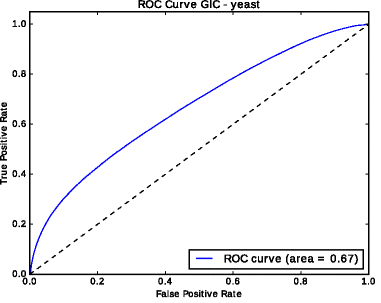
\includegraphics[width=.8\textwidth]{ppi1.png}}
\end{frame}

\begin{frame}
  \frametitle{Applications of semantic similarity}
  \centerline{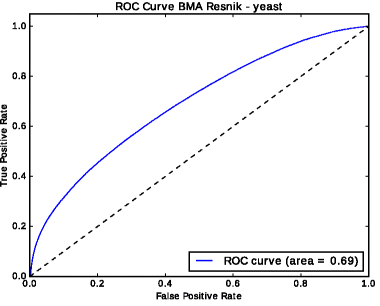
\includegraphics[width=.8\textwidth]{ppi2.png}}
\end{frame}

\begin{frame}
  \frametitle{Applications of semantic similarity}
  \centerline{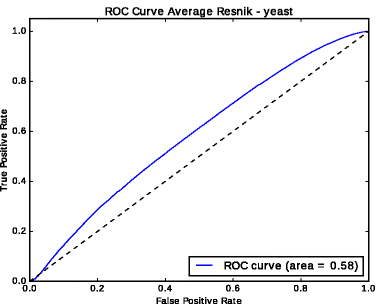
\includegraphics[width=.8\textwidth]{ppi3.png}}
\end{frame}

\begin{frame}
  \frametitle{Applications of semantic similarity}
  Recommendations:
  \begin{itemize}
  \item use Resnik's information content measure
  \item use Resnik's similarity
  \item use Best Match Average
  \item use the full ontology
  \item $\Rightarrow$ but there are many exceptions
    \begin{itemize}
    \item similar location $\Rightarrow$ use location subset of GO
    \item developmental phenotypes $\Rightarrow$ use developmental
      branch of phenotype ontology
    \end{itemize}
  \end{itemize}
\end{frame}

\begin{frame}
  \frametitle{Applications of semantic similarity}
  \begin{itemize}
  \item choice of ontology determines the kind of similarity
  \item functional similarity: Gene Ontology
  \item anatomical, structural similarity: anatomy ontologies (Uberon,
    MA, FMA, etc.)
  \item phenotypic similarity: phenotype ontology (HPO, MP, etc.)
  \item chemical structural similarity: ChEBI
  \end{itemize}
\end{frame}

\begin{frame}
  \frametitle{Applications of semantic similarity}
  \begin{itemize}
  \item phenotypic similarity used to:
    \begin{itemize}
    \item diagnosis: similarity between patient phenotypes and disease
      phenotypes
      \begin{itemize}
      \item also between patient phenotypes and gene--phenotype
        associations
      \item Phenomizer: \url{http://compbio.charite.de/phenomizer/}
      \end{itemize}
    \item disease modules: similarity between disease and disease
    \item clustering/stratification: similarity between patient and patient
    \item disease gene discovery: similarity between patient/disease
      phenotypes and gene--phenotype associations
      \begin{itemize}
      \item in humans
      \item in model organisms
      \end{itemize}
    \item drug repurposing: side-effect similarity; similarity between
      side effect profile and gene--disease associations
    \end{itemize}
  \end{itemize}
\end{frame}



\begin{frame}
  \frametitle{Applications of semantic similarity}
  \centerline{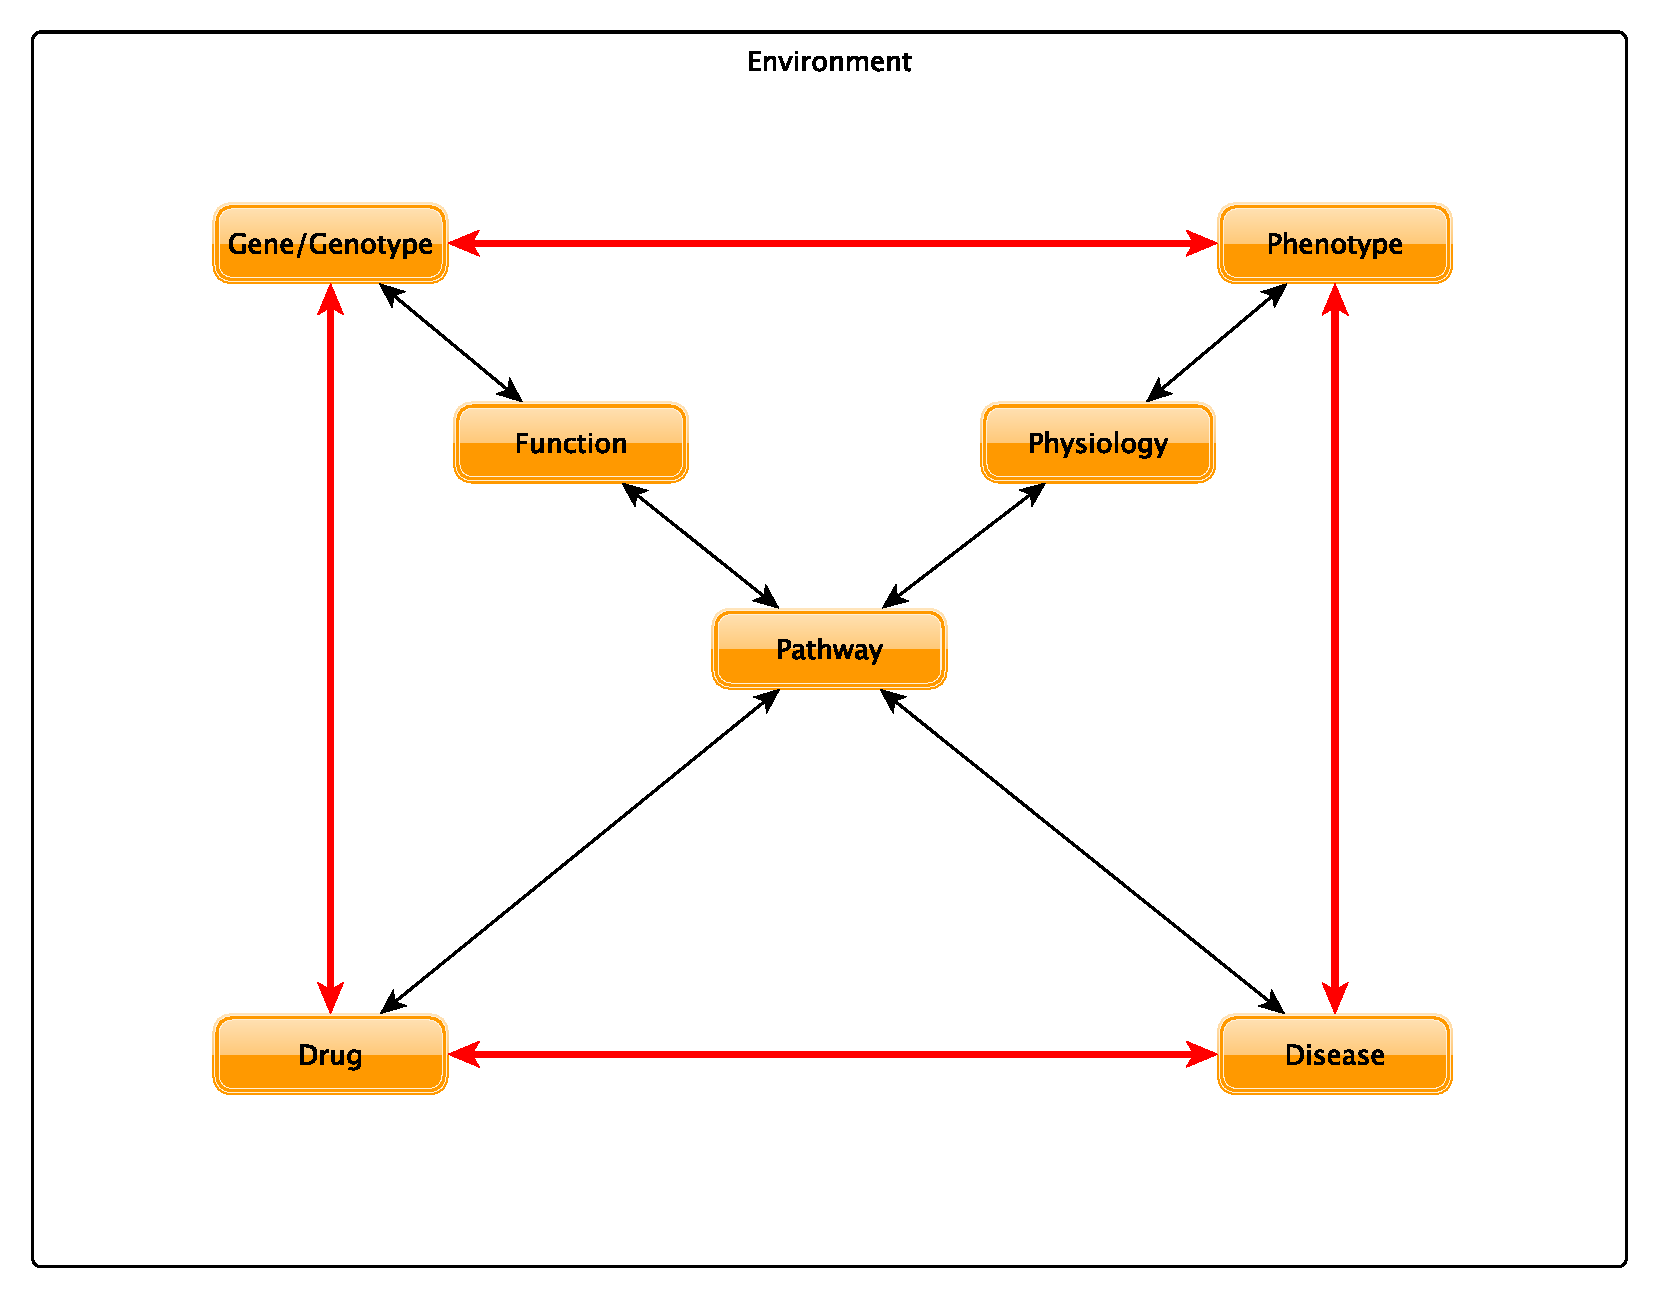
\includegraphics[height=\textheight]{vision1.pdf}}
\end{frame}

\begin{frame}
  \frametitle{Applications of semantic similarity}
  \centerline{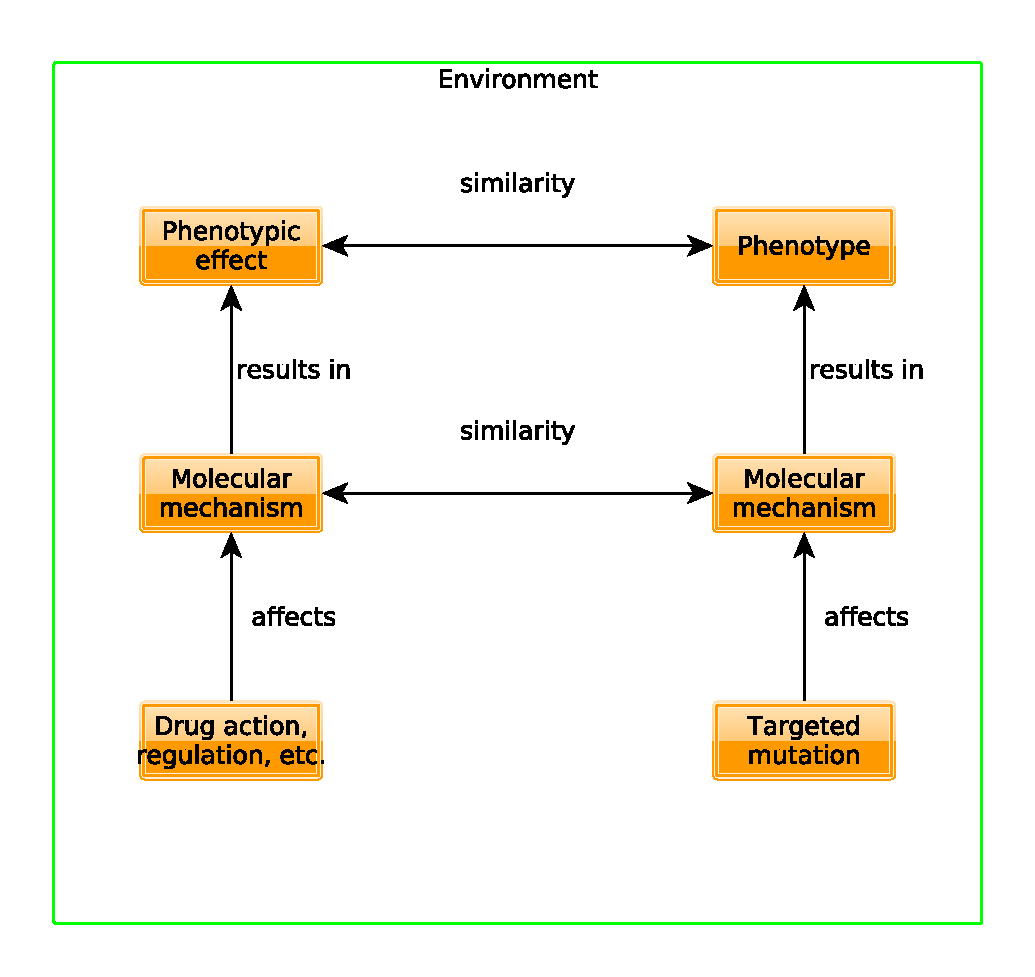
\includegraphics[height=\textheight]{similarity.eps}}
\end{frame}

\begin{frame}
  \frametitle{Applications of semantic similarity}
  \begin{itemize}
  \item Guilt-by-association:
    \begin{itemize}
    \item $x$ is associated with $y$
    \item $z$ is similar to $x$
    \item therefore: $z$ may be associated with $y$
    \end{itemize}
  \item candidate genes (polygenic disease):
    \begin{itemize}
    \item FunSimMat: similar function $\Rightarrow$ similar/same
      disease
    \item side effect similarity: similar side effects $\Rightarrow$
      similar targets/indications
    \end{itemize}
  \end{itemize}
\end{frame}

\begin{frame}
  \frametitle{Applications of semantic similarity}
  \begin{itemize}
  \item No guilt-by-association:
    \begin{itemize}
    \item $x$ causes $a$
    \item $y$ has $b$
    \item $a$ similar to $b$
    \item therefore: $b$ is caused by $x$
    \end{itemize}
  \item candidate genes (monogenic and polygenic disease):
    \begin{itemize}
    \item Phenomizer: gene $x$ causes phenotypes $a$; patient $y$ has
      symptoms $b$; $a$ is similar to $b$; therefore: gene $x$ causes
      the symptoms in $b$
    \item PhenomeNET: similar to Phenomizer but using model organism
      phenotypes (knockouts)
    \item PhenomeDrug: knockout of gene $x$ causes phenotypes $a$;
      drug $y$ causes side effects $b$; $a$ is similar to $b$;
      therefore: drug $y$ inhibits $x$ (or: phenotypes $b$ are caused
      by inhibition of $x$)
    \item needs to compare model organism phenotypes and human
      phenotypes $\Rightarrow$ ontology alignment/integration/mapping
    \end{itemize}
  \end{itemize}
\end{frame}

\begin{frame}
  \frametitle{Applications of semantic similarity}
  \begin{itemize}
  \item comparing entities annotated with {\em different}
    ontologies/vocabularies of the {\em same} (or related) domains
    \begin{itemize}
    \item medical: UMLS, HPO, DO, ORDO, NCIT, ICD, SNOMED CT, MeSH, ...
    \item phenotype: HPO, MP, CPO, WBPhenotype, FBCV, MeSH, ...
    \item chemical: ChEBI, MeSH, DrOn, RXNorm, DrugBank, ...
    \end{itemize}
  \item needs mapping, alignment, or integration
    \begin{itemize}
    \item mapping: given a term $t$, find corresponding class in
      ontology $O$
      \begin{itemize}
      \item can be 1:1, 1:n, n:1, n:m
      \item $t$ can be from ontology, vocabulary, database, or text
      \item use $O$ for analysis
      \end{itemize}
    \item alignment: given two ontologies or vocabularies $O_1$ and
      $O_2$, find all mappings between classes/terms in $O_1$ and $O_2$
      \begin{itemize}
      \item applicable to ontologies and vocabularies
      \item use $O_1$ or $O_2$ for analysis
      \end{itemize}
    \item integration: given two ontologies $O_1$ and $O_2$, combine
      both ontologies into a single ontology $O$
      \begin{itemize}
      \item maintain meaning of classes
      \item use $O$ for analysis
      \end{itemize}
    \end{itemize}
  \end{itemize}
\end{frame}

\begin{frame}
  \frametitle{Applications of semantic similarity}
  \begin{itemize}
  \item lexical mappings: use class labels (and synonyms) to find matches
    \begin{itemize}
    \item hypertension ({\tt HP:0000822}) and hypertension ({\tt MP:0000231})
    \end{itemize}
  \item semantic mappings: use class axioms to find matches
    \begin{itemize}
    \item pulmonary valve stenosis ({\tt MP:0006182}) and Pulmonic
      stenosis ({\tt HP:0001642})
    \item both definitions based on constricted ({\tt PATO:0001847})
      and pulmonary valve ({\tt UBERON:0002146})
    \end{itemize}
  \item hybrid: combine lexical and semantic mappings
  \end{itemize}
\end{frame}

\begin{frame}
  \frametitle{Applications of semantic similarity}
  tools for ontology mapping, matching, integration:
  \begin{itemize}
  \item AgreementMaker Light: \url{https://github.com/AgreementMakerLight/AML-Jar}
    \begin{itemize}
    \item structural (semantic) and lexical matches
    \item can use domain-specific background knowledge
    \end{itemize}
  \item LogMap: \url{https://github.com/ernestojimenezruiz/logmap-matcher}
    \begin{itemize}
    \item structural (semantic) and lexical matches
    \item biology-themed versions
    \end{itemize}
  \item NCBO Annotator: \url{https://bioportal.bioontology.org/annotator}
    \begin{itemize}
    \item lexical matches only
    \item can annotate full text
    \end{itemize}
  \item recent tools and comprehensive ongoing evaluation:
    \begin{itemize}
    \item OAEI: \url{http://oaei.ontologymatching.org/}
    \end{itemize}
  \end{itemize}
\end{frame}

\begin{frame}
  \frametitle{Applications of semantic similarity}
  semantic similarity and text mining:
  \begin{itemize}
  \item find all occurrences of classes of one (or more) ontologies in text
    \begin{itemize}
    \item using lexical matching or semantic annotations
      of text
    \item TextPresso (\url{http://www.textpresso.org/}), NCBO
      Annotator (\url{https://bioportal.bioontology.org/annotator}),
      WhatIzIt (\url{http://www.ebi.ac.uk/webservices/whatizit/info.jsf})
    \item ontology-specific text normalization tools
      \begin{itemize}
      \item DNorm (diseases), GNorm (gene names), OSCAR (chemicals), ...
      \end{itemize}
    \end{itemize}
  \item use for database construction (automatic annotation), relation
    extraction, network construction (co-occurrence network), etc.
  \end{itemize}
\end{frame}

\begin{frame}
  \frametitle{Applications of semantic similarity}
  \centerline{http://aber-owl.net/aber-owl/diseasephenotypes/}
  \begin{itemize}
  \item find phenotypes (signs and symptoms) associated with common
    diseases
    \begin{itemize}
    \item no resource available for comparison
    \end{itemize}
  \item pattern-based mining of literature with Aber-OWL: PubMed
  \item evaluation (of genetically based disease phenotypes) with
    experimentally validated disease genes
  \end{itemize}
\end{frame}

\begin{frame}
  \frametitle{Applications of semantic similarity}
  \framesubtitle{http://aber-owl.net/aber-owl/diseasephenotypes/}
  \centerline{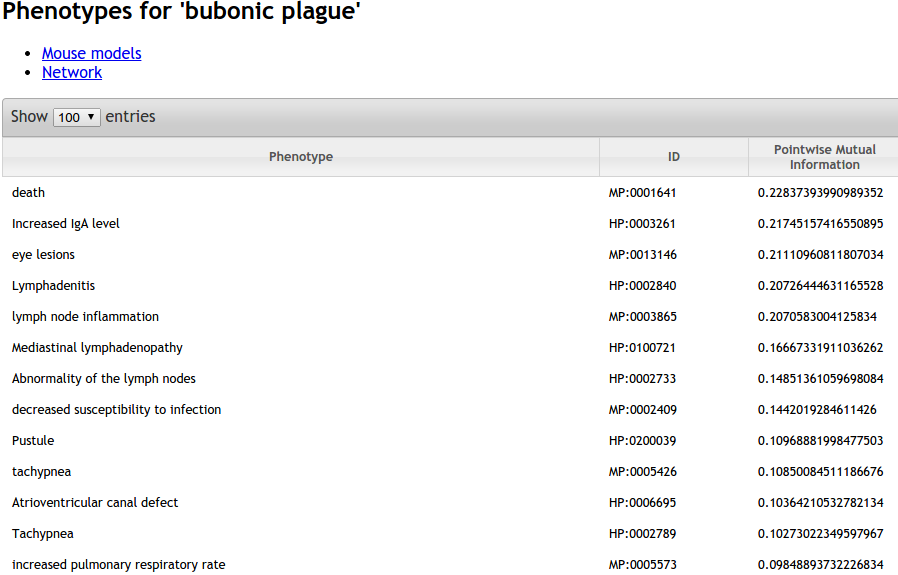
\includegraphics[width=1\textwidth]{aber-owl-plague.png}}
\end{frame}

\begin{frame}
  \frametitle{Applications of semantic similarity}
  \framesubtitle{http://aber-owl.net/aber-owl/diseasephenotypes/}
  \centerline{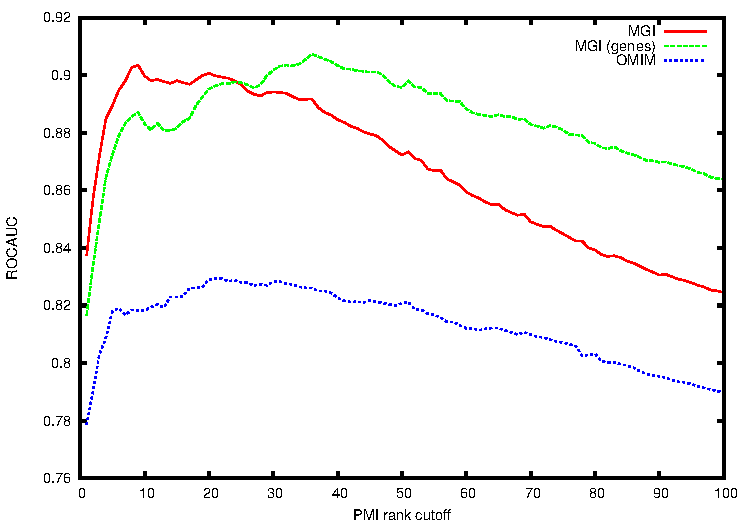
\includegraphics[width=1\textwidth]{pmi-auc-plot.pdf}}
\end{frame}

\begin{frame}[plain]
  \frametitle{Applications of semantic similarity}
  \centerline{\includegraphics[height=1\textheight]{network.eps}}
\end{frame}

\begin{frame}
  \frametitle{Applications of semantic similarity}
  \begin{itemize}
  \item semantic similarity can be used as features in machine
    learning models
    \begin{itemize}
    \item when annotation space is too large
      \begin{itemize}
      \item e.g., GO: 50,000 classes
      \item replace binary representation
      \end{itemize}
    \item to incorporate background knowledge
      \begin{itemize}
      \item semantic similarity encodes {\em implicitly} for ontology
        structure and axioms
      \item encodes for {\em specificity} of classes
      \end{itemize}
    \item negative: reduce all annotations to single value
      \begin{itemize}
      \item leads to loss of information
      \item but is easier to use by many machine learning methods
      \end{itemize}
    \end{itemize}
  \end{itemize}
\end{frame}

\begin{frame}
  \frametitle{Applications of semantic similarity}
  \begin{tikzpicture}[remember picture,overlay]
    \node[at=(current page.center)] {
      \centerline{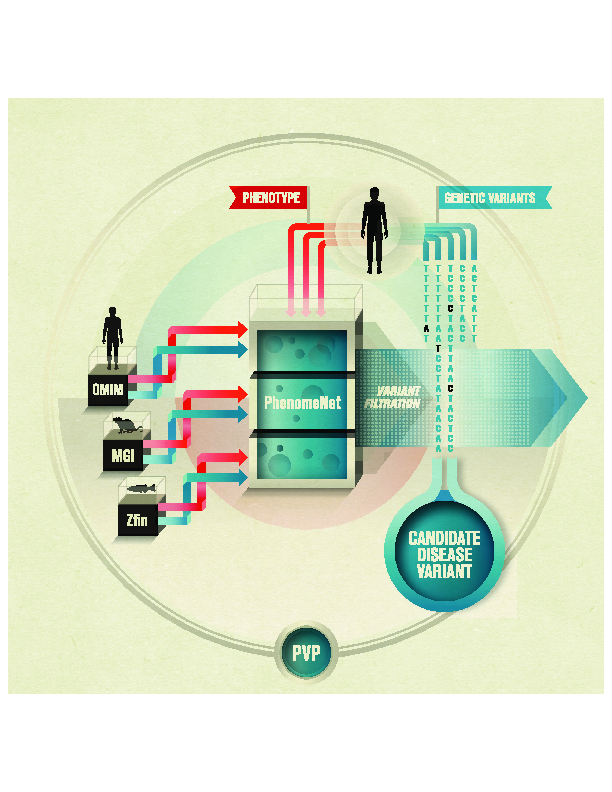
\includegraphics[height=1\textheight]{pvp.pdf}}
    };
  \end{tikzpicture}
\end{frame}

{
\setbeamercolor{background canvas}{bg=}
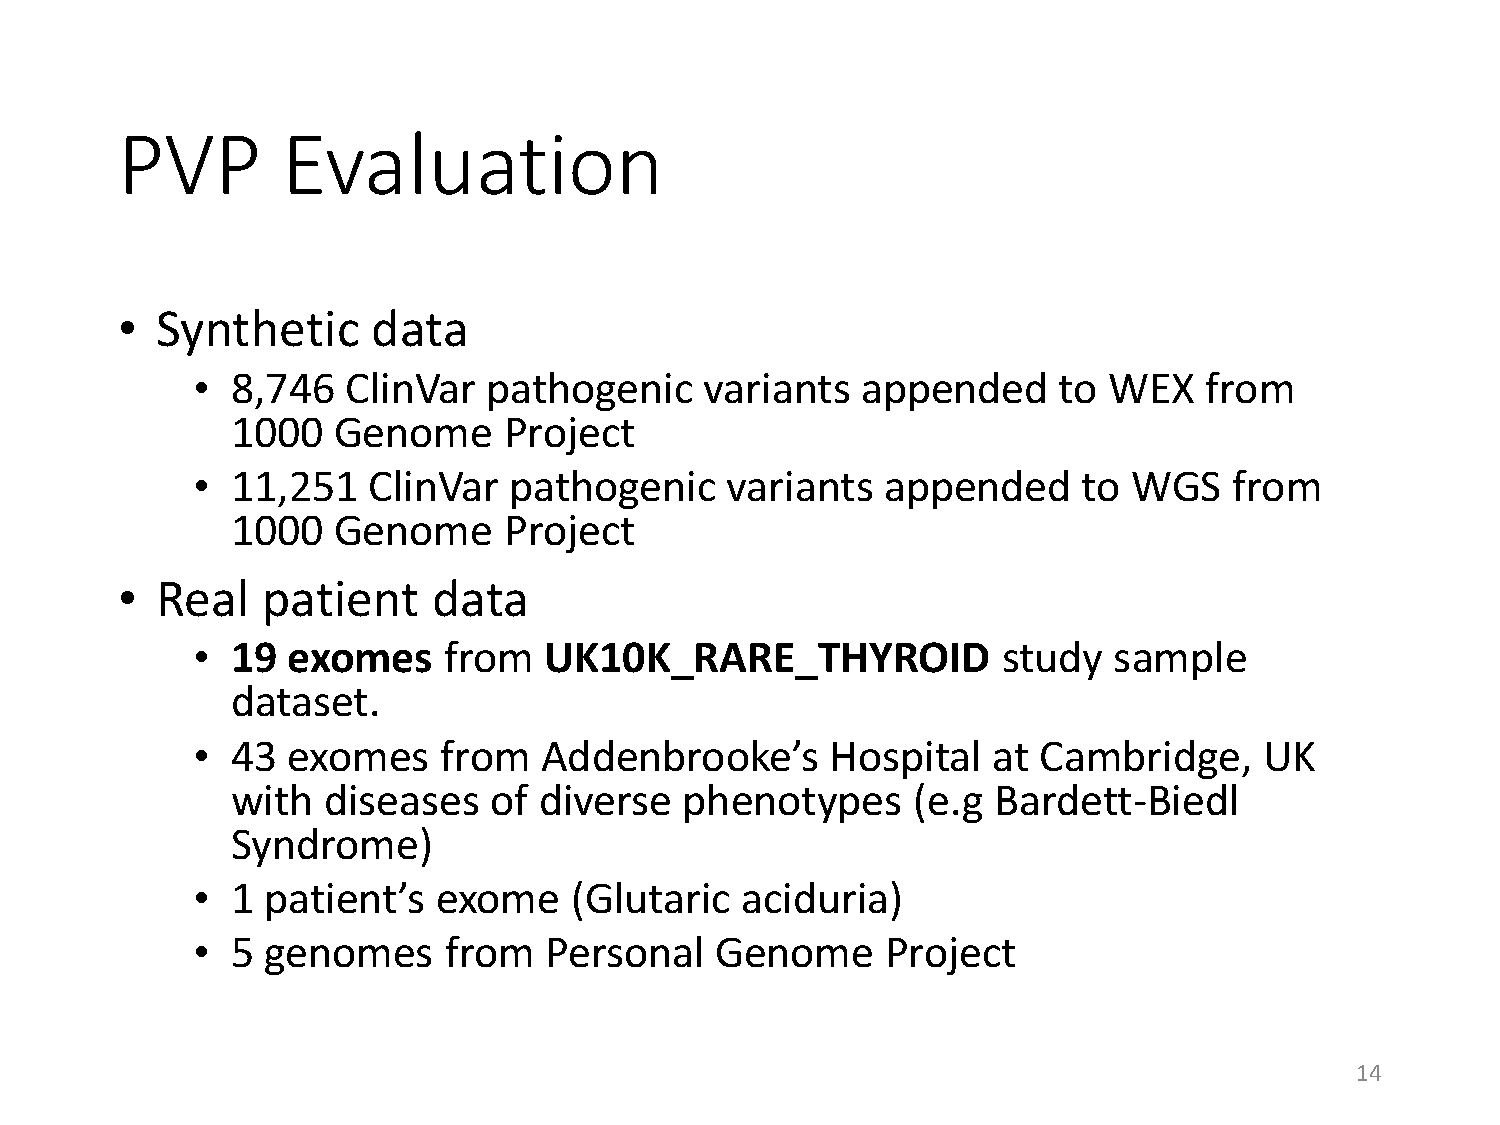
\includepdf[pages=1-3]{hh-pvp2.pdf}
}

\begin{frame}
  \frametitle{Summary}
  \begin{itemize}
  \item many semantic similarity measures
    \begin{itemize}
    \item graph-based
    \item feature-based
    \end{itemize}
  \item useful for similarity-based prediction
    \begin{itemize}
    \item similar entities $\Rightarrow$ guilt-by-association
    \item different entities
    \end{itemize}
  \item combine with data and text mining
  \item features in machine learning methods
  \end{itemize}
\end{frame}

\begin{frame}
  \frametitle{Hands-on: semantic similarity}
  \begin{itemize}
  \item if you have not done so {\em before} the tutorial, don't start now
    \begin{itemize}
    \item you need to download {\em a lot} of data
    \item you can follow in our demonstration
    \end{itemize}
  \item Beaker Notebook
    \begin{itemize}
    \item like iPython Notebook, or Jupyter, with lots of kernels
    \item Python, Groovy, Javascript, ...
    \end{itemize}
  \item
    \url{https://github.com/bio-ontology-research-group/ontology-tutorial}
  \end{itemize}
\end{frame}

\begin{frame}
  \frametitle{Hands-on: semantic similarity}
  In the tutorial, we will
  \begin{itemize}
  \item download an ontology
  \item explore the ontology with OWLAPI
  \item classify the ontology with an OWL reasoner
    \begin{itemize}
    \item and query using an OWL reasoner
    \end{itemize}
  \item store the inferred version locally
  \item use the Semantic Measures Library to:
    \begin{itemize}
    \item explore the ontology as graph
    \item compute similarity between classes
    \item use different similarity measures
    \item compare patients to mice
    \end{itemize}
  \item you can build on this and extend for your own research!
  \end{itemize}
\end{frame}

\end{document}
%%% Local Variables:
%%% mode: latex
%%% TeX-master: t
%%% End:
